Bitcoin was not created in a vacuum and to understand the design of Bitcoin and by extension the Lightning Network one would
benefit from understanding money and systems of trust. Nakamoto encoded "the times 03/jan/2009 chancellor on brink of second bailout for banks"\cite{repository:bitcoin:sourceforge}\cite{bitcoin:genesis:coinbase} in coinbase transaction of the genesis block as an alleged comment on the current banking system as well as a time stamp. He later cemented this view with multiple forum posts while he still was active.

\subsection{Origin of money}

On the fringes of our specie barter became the first
medium in which trade became22 viable, removing the risk 
from otherwise simple delayed reciprocity. It is possible
for a trade to be mutual beneficial as Nick Szabo 
se elegantly explained:

\begin{displayquote}

"individuals, clans, and tribes all vary in their preferences, vary in their ability to satisfy these preferences, and vary in the beliefs they have about these skills and preferences and the objects that are consequent of them, there are always gains to be made from trade."\cite{szabo:shelling:out}

\end{displayquote}

Barter is by itself quite limiting, consider a System \textbf{S}
consisting of \textbf{n} commodities, the amount of possible exchanges
between commodities in \textbf{S} is \textbf{n x n}. When \textbf{n} increases, the exchange pairs explodes exponentially.
This makes it difficult asses fair pricing and decreases the coincidence of a trade\footnote{The coincidence of finding another party who is looking to exchange the same commoditiy pair you are but in reverse order.}. 
The economist Carl Menger described it as inevitable for money to evolve from a sufficient volume of
commodity barter\cite{menger:origins:money}. If the same System \textbf{S} is considered with money - the possible exchange pairs would be reduced to only \textbf{n} pairs. 

\subsubsection{Characteristics of money}

Out of these commodities money emerged and history has provided many peculiar forms of money. The Rai stones of Yap islands, The Wampun shells in North America\footnote{The wampun shells were actually legal tender as recently as 1710 in North Carolina and long into the 1600s in New England.}\cite{szabo:shelling:out} and Aggry beeds to name a few. Although many different types of commodities have acted as money during certain time in history there are some properties that seem favorable and recur. X has x list:

list

Many of the previous mentioned monies have expressed many these properties well. Changes in these properties have also lead to there downfall. Rai stones are carved limestone which are not native to the Yap islands, when outsiders started to bring in these on large ships it quickly changed their stock-to-flow ratio for the worst\cite{ammous:bitcoin:standard}. Aggry beeds met the same fate when Europeans started to export them to Africa and modern shell fishing ruined the Wampun shells function as money\cite{szabo:shelling:out}.

Rare metals have held these attributes since the beginning of history and in many ways still hold them today.

\subsection{Bearer promissory notes}

Although gold emerged as the commodity best suited as money
it still had two major problems:

\begin{enumerate}
	\item Gold is unsuitable for small transactions due to the limit in divisibility.
	\item Gold is expensive to carry around and protect.
\end{enumerate}

Private and central banks began to issue bearer promissory notes to the owners of the underlying asset it stored(e.g figure \ref{fig:seb:promissory:note}). 
The asset could then be retrieved for the note on demand. The notes themselves could then be traded 
instead of the underlying gold. This solved both the above problems, notes are easy to carry, conceal and 
could be minted in very small amounts. 

\begin{figure}[!htb]
	\centering
	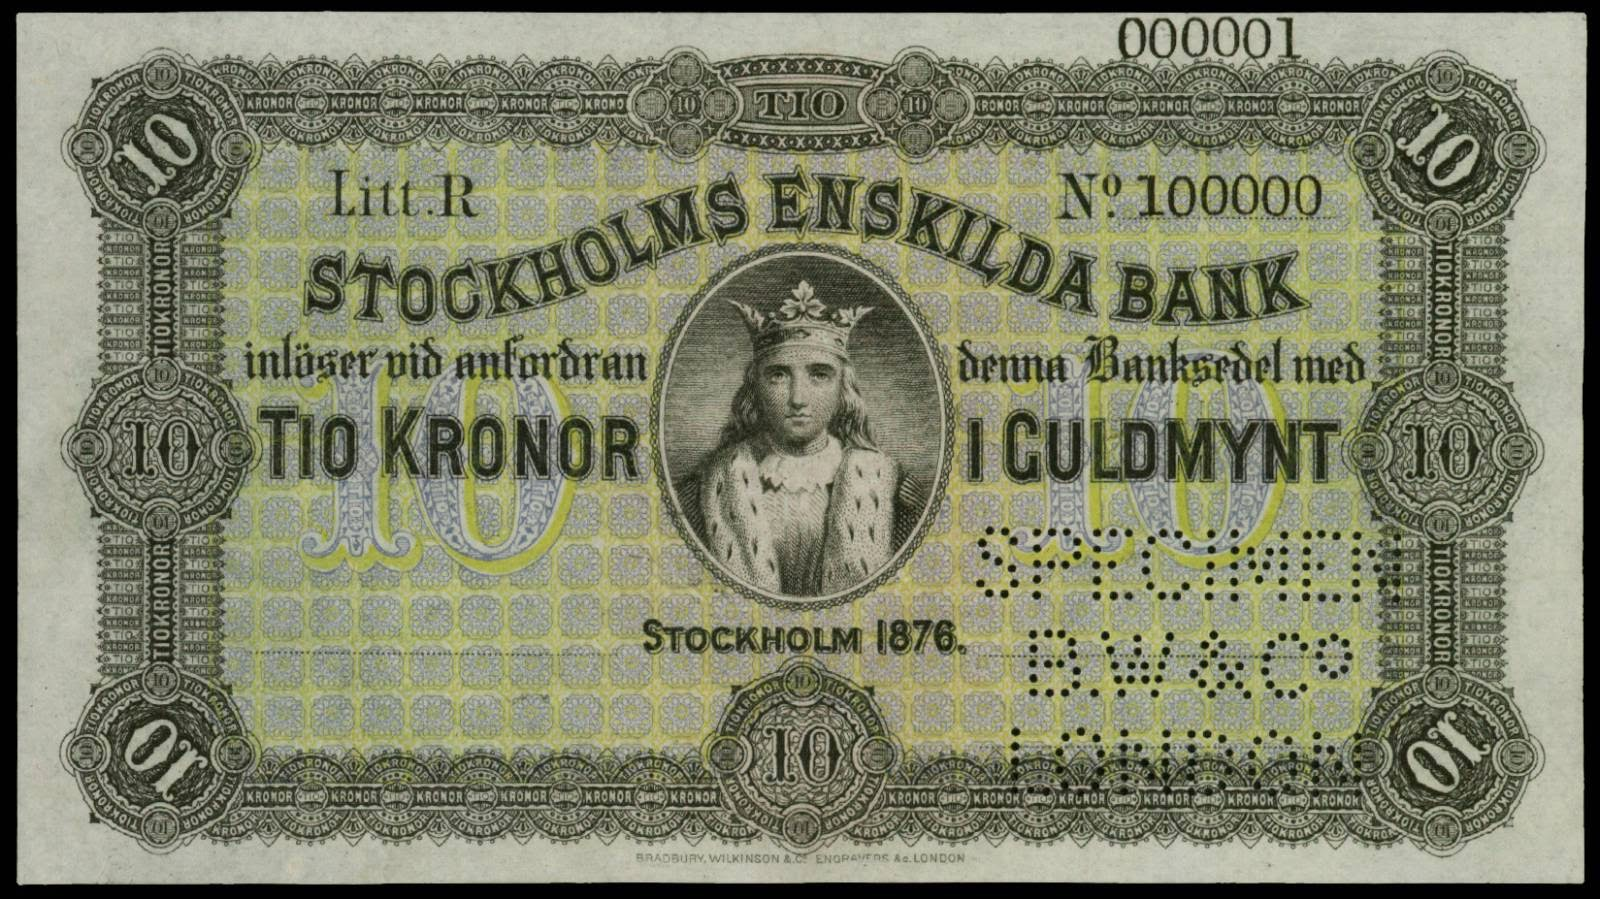
\includegraphics[width=7cm]{PrivateBankNoteStockholmEnskildaBank1876.JPG}
	\caption{\textit{The private bank 'Stockholms Enskilda Bank'(SEB) issued bearer
	promissory note. It promises to pay 10 crowns to the bearer upon demand in gold. 
	The exchange rate as per the Scandinavian Convention(Sweden, Denmark 27 may 1873, Norway 1 april 1877)\cite{nordic:crown}
	was 1 kilogram gold per 2480 crowns or 1 crown per 0.403g gold\cite{crown:gold}. 
 }}
	\label{fig:seb:promissory:note}
\end{figure}

By the late 19th century almost all major currencies was under the gold standard as seen in table \ref{tab:gold:standard}.

\begin{table}[!htb]
	\begin{tabular}{lllll}
		Nation & Currency & Period & Years \\
		France & Franc & 1814-1914 & 100 \\
		Netherlands & Guilder & 1816-1914 & 98 \\
		G.Britain & P. Sterling & 1821-1914 & 93 \\
		Switzerland & Franc & 1850-1936 & 86 \\
		Belgium & Franc & 1832-1914 & 82 \\
		Sweden & Kronor & 1873-1931 & 58 \\
		Germany & Mark & 1875-1914 & 39 \\
		Italy & Lira & 1883-1914 & 31 \\   
	\end{tabular}
	\caption{\textit{ Major European nations periods under the gold standard
			as composed by Ferdinand Lips\cite{lips:gold:wars} from 1975 Pickís Currency Yearbook data.
	}}
	\label{tab:gold:standard}
\end{table}

\subsubsection{Bank runs}

The introduction of the promissory note solved the two previously mentioned problems but also 
introduced trust.\footnote{Note that this a much wider problem than for only promissory notes. This trust model is what makes banks in the first place.} 

Although the gold deposits could be regularly audited by a third party there is little to no guarantee that the bank in question wouldn't issue more notes than gold it holds in reserve. Banks utilizing this sort of practice could go on for a very long time before getting caught. Consider a bank that issue twice as many notes as it holds gold in reserve. It would require 50\% of it's notes to be demanded for the bank to default.  
  
There has been many so called bank runs in history. The public gets suspicious in the bank and the trust disappear - leading to massive withdrawals in a short time span. Even if banks are technically solvent, having assets tied up in different ventures, they could fail to deliver on the notes promises. This can also be viewed as a negative spiral, people start to withdraw, increasing the risk of default, more people start to withdraw due to the higher risk. R.H. Patterson elaborates in detail the bank run in Great Britain in 1866 leading to the default of Overend, Gurney and Company and the behavior under panic: 

\begin{displayquote}
	"When a Panic occurs, a much more serious home-drain is produced upon the bank. At such time cheques fall somewhat into disrepute, so that merchants in some cases require payment in cash. The public also, to some extent, take to hoarding[...]. But a very large part of the drain upon the Bank of England in the form of hoarding ,[...],is made by other banks: for these banks being liable to unusual demands on the part of their customers, have to keep in hand a larger stock of money than usual"\cite{patterson:monetary:drains}
\end{displayquote}

Overall most larger institutions stayed solvent and bank runs is more an exception than a rule during this time period. Since all major currencies were denominated in gold the threshold for global trade sank. During the gold standard era the economy boomed with trade and is often known under the French term 'Belle Epoque' or 'Beautiful era'. 

\subsection{Elasticity of money}

It all came crashing down with the 

\newpage
\onecolumn
\begin{figure}[!htb]
	\centering
	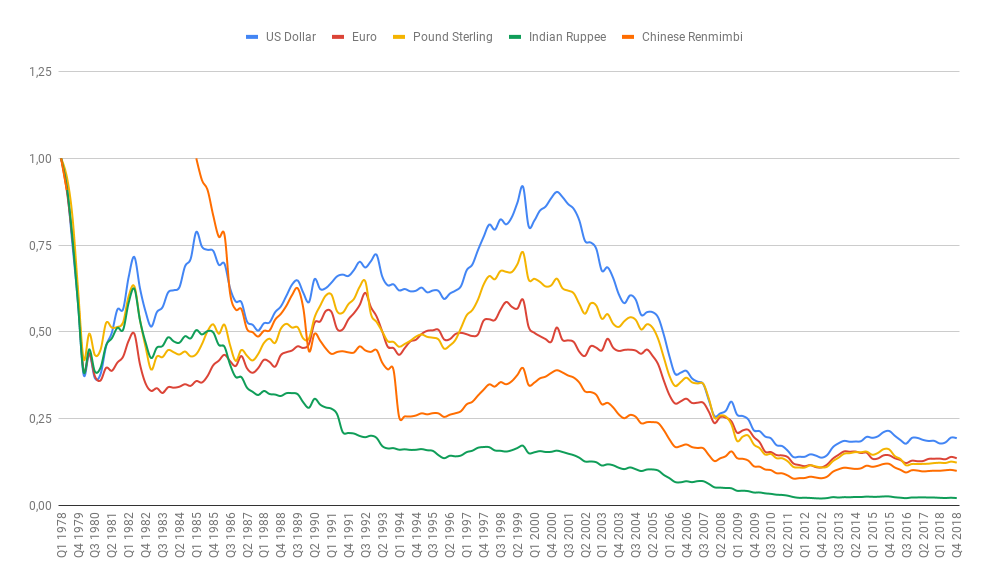
\includegraphics[width=16cm]{gold-price.png}
	\caption{\textit{The relation of major currencies against it's value in gold since the end of the Bretton Woods agreement to
			today. The graph is composed with data from the World Gold Council\cite{world:gold:council}. 
	}}
	\label{fig:seb:promissory:note}
\end{figure}
\twocolumn


\subsection{Relevancy}
In many ways it help to think of bitcoin
as both a bearer instrument and as a monetary system and how the 
system is designed as such. This
section is an incomplete view on it's own and for
further reading these recommendations are good starting points: 

\begin{itemize}
	\item Nick Szabo's blog Enumerated and above cited Shelling out\cite{szabo:shelling:out}.
	\item Saifedean Ammous's The bitcoin standard.\cite{ammous:bitcoin:standard}
\end{itemize}